\documentclass[onecolumn,superscriptaddress,amsmath,amssymb,longbibliography]{revtex4-2}

\usepackage{graphicx}
\graphicspath{{../figures/}}
\usepackage{booktabs}
\usepackage{multirow}
\usepackage{hyperref}

% Custom commands matching main paper
\newcommand{\cert}[1][]{\mathcal{C}_{#1}}
\newcommand{\xc}{\mathrm{xc}}
\newcommand{\conv}{\mathrm{conv}}
\newcommand{\meth}{\mathrm{meth}}
\newcommand{\Ecut}{E_{\mathrm{cut}}}
\newcommand{\Nk}{N_k}
\renewcommand{\thefigure}{S\arabic{figure}}
\renewcommand{\thetable}{S\arabic{table}}
\renewcommand{\theequation}{S\arabic{equation}}

\begin{document}

\title{Supplemental Material for ``A Posteriori Error Certificates (APECs): Certifying Uncertainty Through the Soft-Mode Bottleneck in BaTiO$_3$''}

\author{Julien Appleby-Millette}
\affiliation{Department of Chemistry and the Centre for Advanced Materials and Related Technology, University of Victoria, Victoria, British Columbia V8W 2Y2, Canada}
\author{Kyla Younger}
\affiliation{Department of Chemistry and the Centre for Advanced Materials and Related Technology, University of Victoria, Victoria, British Columbia V8W 2Y2, Canada}
\author{Thomas Baker}
\affiliation{Department of Physics and Astronomy, University of Victoria, Victoria, British Columbia V8W 2Y2, Canada}
\affiliation{Department of Chemistry, University of Victoria, Victoria, British Columbia V8W 2Y2, Canada}
\author{Irina Paci}
\affiliation{Department of Chemistry and the Centre for Advanced Materials and Related Technology, University of Victoria, Victoria, British Columbia V8W 2Y2, Canada}

\date{\today}

\maketitle

This Supplemental Material provides extended formalism
(Sections~\ref{sec:si_covariance}--\ref{sec:si_convergence_est}), the
certificate schema specification (Section~\ref{sec:si_schema}), supporting
data tables (Section~\ref{sec:si_tables}), the complete BaTiO$_3$ literature
library (Section~\ref{sec:si_library}), certificate data
(Section~\ref{sec:si_certs}), and the extraction case study
(Section~\ref{sec:si_extraction}). It also records the independent SCF
convergence campaign used to check the cutoff and $k$-mesh behavior of the
40-atom BaTiO$_3$ supercell and the leave-one-out calibration check used to
test the certificate uncertainties. Schematic downstream process-chain and
residual-diagnostic examples are included to clarify how the schema can be
extended without treating those extensions as completed main-text results.

%%%%%%%%%%%%%%%%%%%%%%%%%%%%%%%%%%%%%%%%%%%%%%%%%%%%%%%%%%%%%%%%%%%%%%%%%%%%%%%
\section{S1. Extended Formalism}
%%%%%%%%%%%%%%%%%%%%%%%%%%%%%%%%%%%%%%%%%%%%%%%%%%%%%%%%%%%%%%%%%%%%%%%%%%%%%%%

\subsection{S1.1. Diagonal and Covariance-Aware Fusion}
\label{sec:si_covariance}

The main text uses two related covariance approximations. First, within a
single certificate, the reported convergence, methodological, intrinsic DFT,
and model-form components are combined with a diagonal covariance
approximation unless material-specific covariance data are available. Second,
when multiple certified entries are fused, the default inverse-variance
weighted (IVW) estimator assumes that the entries are exchangeable and
conditionally independent after phase, tensor-component, and target-observable
partitioning.

For observations collected in a vector
$\mathbf{y}=(P_1,\ldots,P_n)^{\mathsf T}$ with covariance matrix $\Sigma$, the
generalized least-squares fused estimate is
\begin{equation}
    \hat{P}_{\mathrm{GLS}} =
    \frac{\mathbf{1}^{\mathsf T}\Sigma^{-1}\mathbf{y}}
         {\mathbf{1}^{\mathsf T}\Sigma^{-1}\mathbf{1}},
    \qquad
    \sigma_{\mathrm{GLS}}^2 =
    \frac{1}{\mathbf{1}^{\mathsf T}\Sigma^{-1}\mathbf{1}} .
\end{equation}
If $\Sigma$ is diagonal, this reduces to the IVW rule used in the BaTiO$_3$
case study. If source-level correlations are known or can be estimated, they
should enter as off-diagonal terms. Examples include shared pseudopotentials,
shared training/calibration sets, copied benchmark values, identical
functional families, or multiple records generated by the same workflow.

When correlations are suspected but not yet quantified, the conservative
certificate behavior is to partition more aggressively and avoid claiming
spurious precision. A useful diagnostic is the effective sample size
\begin{equation}
    N_{\mathrm{eff}} =
    \frac{(\sum_i w_i)^2}{\sum_{ij} w_i w_j R_{ij}},
\end{equation}
where $w_i$ are scalar fusion weights and $R_{ij}$ is the correlation matrix.
For independent entries, $R$ is the identity and $N_{\mathrm{eff}}$ approaches
the usual Kish effective sample size; for strongly correlated entries,
$N_{\mathrm{eff}}$ can be much smaller than the count of records. This is the
formal version of the main-text caution that literature and database fusion
should not treat every row as a new independent experiment.

\subsection{S1.2. Hierarchical Bayesian Fusion}
\label{sec:si_bayesian}

The inverse-variance weighting and bias-corrected fusion methods described in
the main text assume that systematic biases are either negligible or known.
When biases are uncertain or material-dependent, hierarchical modeling treats
them as draws from a population distribution \cite{Kennedy2001,Sivia2006}:
\begin{align}
    P_i | P_{\mathrm{true}}, \beta_i &\sim \mathcal{N}(P_{\mathrm{true}} + \beta_i, \sigma_i^2) \\
    \beta_i &\sim \mathcal{N}(\mu_\beta, \tau_\beta^2) \\
    P_{\mathrm{true}} &\sim \mathcal{N}(\mu_0, \sigma_0^2)
\end{align}
where $P_i$ is the $i$-th estimate, $\beta_i$ its functional-specific bias,
$\sigma_i$ its reported uncertainty, and $(\mu_\beta, \tau_\beta)$ are
hyperparameters governing the bias distribution. The prior on
$P_{\mathrm{true}}$ can be uninformative ($\sigma_0 \to \infty$).

The posterior $p(P_{\mathrm{true}} | \{P_i\})$ can be computed analytically for
this conjugate Gaussian model. When the bias hyperparameters are unknown, they
can be estimated from the data (empirical Bayes) or sampled via MCMC for fully
Bayesian inference.

This approach is particularly valuable when fusing data across functionals
(LDA, PBE, hybrid) that have known systematic tendencies: LDA overbinds, PBE
underbinds, and the bias magnitude varies by material class. The hierarchical
model automatically downweights estimates whose bias is large relative to the
population, without requiring prior knowledge of individual biases.

The main text exercises the simpler inverse-variance weighting (appropriate
when biases are small relative to random uncertainties). The hierarchical
model becomes important when fusing across functionals with strongly different
systematic tendencies---a regime that arises naturally as the certificate
framework scales to multi-material, multi-functional databases.


\subsection{S1.3. Monte Carlo Propagation}
\label{sec:si_mc}

For derived quantities $Q = f(P_1, P_2, \ldots, P_n)$ where the linear
propagation formula in the main text breaks down due to nonlinearity or
large relative uncertainties, Monte Carlo sampling provides robust estimates:
\begin{equation}
    Q^{(k)} = f(P_1^{(k)}, \ldots, P_n^{(k)}), \quad
    P_i^{(k)} \sim \mathcal{N}(\hat{P}_i, \sigma_{P_i}^2)
\end{equation}
for $k = 1, \ldots, K$ samples. The distribution of $\{Q^{(k)}\}$ provides
the full posterior, from which mean, standard deviation, percentiles, and
skewness can be extracted.

This approach is consistent with the Monte Carlo method for uncertainty
evaluation recommended by the Guide to the Expression of Uncertainty in
Measurement \cite{JCGM2008_GUM,JCGM2008_MC,Possolo2015}. For the
BaTiO$_3$ case study, the soft-mode model $r_{33} \propto
Z^{*2}/(\varepsilon \omega^2)$ is sufficiently nonlinear (with $\gamma =
\pm 2$ exponents) that Monte Carlo propagation would capture asymmetric
uncertainty distributions---e.g., when $\omega_{\mathrm{soft}}$ is near the
phase transition and its distribution is skewed. The main text uses linear
propagation, which is adequate for the current parameter regime (3--8\%
input uncertainties). Monte Carlo propagation is the schema-supported route
for certificates outside this linear regime, including cases where
$\omega_{\mathrm{soft}}$ approaches zero and relative uncertainty summaries
become ill-conditioned.


\subsection{S1.4. Multi-Stage Process Chains}
\label{sec:si_chains}

Real computational workflows involve sequential stages, each with its own
certificate:
\begin{equation}
    \boxed{\text{DFT}} \xrightarrow{\cert[1]}
    \boxed{\text{Property}} \xrightarrow{\cert[2]}
    \boxed{\text{Model}} \xrightarrow{\cert[3]}
    \boxed{\text{Prediction}}
\end{equation}
Uncertainties compound through the chain as
\begin{equation}
    \sigma_{\mathrm{final}}^2 = \sigma_1^2 \cdot G_1^2 + \sigma_2^2 \cdot G_2^2 +
    \sigma_3^2
\end{equation}
where $G_i = \partial(\text{stage } i+1)/\partial(\text{stage } i)$ are
sensitivity (gain) factors. This formulation makes explicit where in a pipeline
uncertainty reduction efforts will have the greatest impact. The main text
demonstrates stages 1--2 (DFT $\to$ property $\to$ derived $r_{33}$) and
discusses how the same certificate decomposition can be propagated to device
metrics such as $V_\pi L$ and switching energy.

For electro-optic modulator design, the certified bulk or single-domain
Pockels coefficient is not the end of the uncertainty chain. The response must
pass through additional modeling stages such as domain averaging, waveguide
geometry, optical--RF overlap, propagation loss, and fabrication tolerances.
For example, the common half-wave voltage--length product is
\begin{equation}
    V_\pi L = \frac{\lambda d}{2 n^3 r_{\mathrm{eff}} \Gamma},
    \label{eq:si_VpiL}
\end{equation}
where $\lambda$ is wavelength, $d$ is electrode gap, $n$ is refractive index,
$r_{\mathrm{eff}}$ is the effective Pockels coefficient, and $\Gamma$ is the
optical--RF field overlap \cite{Wooten2000,Reed2010,Wang2018_LN_thin}. Each of
these terms is a candidate certificate target once the corresponding
microstructure, optical-mode, and fabrication models are specified.

The following schematic chain is therefore a schema demonstration, not a
completed device calculation. The DFT and Property stages use the uncertainty
decomposition developed in the main text; the Effective and Device stages are
schematic estimates showing where additional certified domain, strain,
geometry, overlap, and loss models would enter if their exchangeability
classes and model discrepancies were specified.

\begin{center}
\textbf{Illustrative multi-stage uncertainty propagation from DFT to
downstream response-model priors.}\\[0.5em]
\begin{tabular}{llcc}
\toprule
Stage & Quantity & Value & Rel.\ uncertainty \\
\midrule
DFT & $\omega_{\mathrm{soft}}$ & 172 cm$^{-1}$ & 10\% \\
$\downarrow$ ($\times 2$ amplification) & & & \\
Property (single calc) & $r_{33}$ ($zz$) & 94 pm/V & 28\% \\
Property (library-fused) & $r_{33}$ ($zz$) & 94 pm/V & 24\% \\
\midrule
\multicolumn{4}{l}{\textit{Downstream stages to be certified:}} \\
$\downarrow$ (microstructure averaging) & & & \\
Effective & $r_{\mathrm{eff}}$ & $\sim$40 pm/V & $\sim$26\% \\
$\downarrow$ (device model) & & & \\
Device & $V_\pi L$ & $\sim$2.5 V$\cdot$cm & $\sim$27\% \\
\bottomrule
\end{tabular}
\end{center}

The current propagation chain does not capture optical propagation loss, which
Kim and Demkov \cite{Kim2025_loss} have shown can be dominated by
non-absorptive scattering at ferroelectric domain walls in BaTiO$_3$
waveguides. Loss is therefore a separate out-of-scope target observable rather
than a contribution that can be folded into $r_{\mathrm{eff}}$ or $V_\pi L$
without its own certificate.


\subsection{S1.5. Convergence Uncertainty Estimators}
\label{sec:si_convergence_est}

The main text defines the total convergence uncertainty as the quadrature sum
$\sigma_\conv^2 = \sigma_{\Ecut}^2 + \sigma_k^2 + \sigma_{\mathrm{SCF}}^2 +
\cdots$. Here we provide the detailed estimators for each component.

For the plane-wave cutoff, the uncertainty combines the estimated truncation
error at the working cutoff with the sensitivity of the property to cutoff
changes:
\begin{equation}
    \sigma_{\Ecut}^2 = \left(\frac{\partial P}{\partial \Ecut}\right)^2
    \cdot \delta E^2 + \epsilon_{\Ecut}^2(E_{\mathrm{used}})
\end{equation}
where $\delta E$ is the step size in the convergence test and
$\epsilon_{\Ecut}(E) = A_E \exp(-E/E_0)$ is the parametric truncation error
model.

For $k$-point sampling, the uncertainty includes a term for anisotropic
sampling effects:
\begin{equation}
    \sigma_k^2 = \epsilon_k^2(\Nk) + \sigma_{\mathrm{symmetry}}^2
\end{equation}
where $\epsilon_k(\Nk) = B/\Nk^\alpha$ and
$\sigma_{\mathrm{symmetry}}$ captures the spread in equivalent-by-symmetry
quantities (e.g., $\sigma_{ii}$ tensor components in a nominally cubic system).

The self-consistency contribution is estimated from the sensitivity of the
property to the residual density at the final SCF iteration:
\begin{equation}
    \sigma_{\mathrm{SCF}} \approx \left|\frac{\partial P}{\partial \rho}\right|
    \cdot \delta\rho_{\mathrm{final}}
\end{equation}
where $\delta\rho_{\mathrm{final}}$ is the SCF residual norm.

\subsubsection*{Residual-Based Diagnostic Indicators}

Several quantities available from a single calculation can provide qualitative
convergence flags when explicit convergence sweeps are unavailable. These
indicators are not used as calibrated uncertainty contributions in the main
BaTiO$_3$ certificate; they are optional diagnostic metadata for automated
certificate generation.

The decay rate of SCF residuals,
\begin{equation}
    r_{\mathrm{SCF}} = \frac{\log(\delta\rho_1 / \delta\rho_N)}{N},
    \label{eq:si_scf_rate}
\end{equation}
indicates electronic-structure conditioning. Slow convergence, for example
$r_{\mathrm{SCF}} < 0.5$, suggests a difficult electronic structure and may
motivate a conservative tier downgrade when no explicit convergence data are
available.

The spread of stress tensor eigenvalues in nominally symmetric systems,
\begin{equation}
    \Delta\sigma = \max_i(\sigma_{ii}) - \min_i(\sigma_{ii}),
    \label{eq:si_stress_spread}
\end{equation}
can flag anisotropic sampling or incomplete relaxation. Non-zero forces at
equilibrium positions similarly indicate incomplete relaxation, basis-set
incompleteness, or a mismatch between the claimed symmetry and the actual
calculated structure.


%%%%%%%%%%%%%%%%%%%%%%%%%%%%%%%%%%%%%%%%%%%%%%%%%%%%%%%%%%%%%%%%%%%%%%%%%%%%%%%
\section{S2. Certificate Schema Specification}
\label{sec:si_schema}
%%%%%%%%%%%%%%%%%%%%%%%%%%%%%%%%%%%%%%%%%%%%%%%%%%%%%%%%%%%%%%%%%%%%%%%%%%%%%%%

\subsection{S2.1. JSON Schema}

The certificate schema is defined as a JSON-serializable structure. A compact
example for a typed BaTiO$_3$ optical-gap certificate is:

\begin{verbatim}
{
  "property": {
    "name": "band_gap",
    "target_observable": "optical_absorption_onset",
    "value": 3.08,
    "unit": "eV"
  },
  "uncertainties": {
    "convergence": 0.096,
    "methodological": 0.462,
    "intrinsic_dft": 0.246,
    "model_form": 0.246,
    "total": 0.585,
    "relative_total": 0.190
  },
  "quality_tier": "RED",
  "exchangeability_key": {
    "material": "BaTiO3",
    "phase": "tetragonal",
    "target_observable": "optical_absorption_onset",
    "temperature_regime": "room_temperature"
  },
  "provenance": {
    "evidence_set": "literature_proxy_plus_optical_anchor",
    "included_targets": ["TB-mBJ_gap", "HSE06_gap",
                         "optical_absorption_onset"],
    "excluded_targets": ["LDA_Kohn-Sham_gap", "PBE_Kohn-Sham_gap"],
    "exclusion_reason": "non_exchangeable_target_observable"
  },
  "fusion": {
    "method": "typed_inverse_variance",
    "covariance_policy": "diagonal_until_source_correlations_available",
    "effective_sample_size": null
  },
  "descriptor_selection": {
    "mode_identification": "not_applicable",
    "selected_descriptor": "optical_absorption_onset"
  },
  "model_discrepancy": {
    "discrepancy_provenance": "referenced",
    "carried_magnitude": 0.246,
    "status": "carried_not_corrected"
  }
}
\end{verbatim}

Key fields:
\begin{itemize}
    \item \texttt{property.target\_observable}: the physical or computational
    quantity being certified; this prevents semilocal Kohn--Sham gaps,
    quasiparticle gaps, and optical onsets from being fused accidentally.
    \item \texttt{uncertainties.model\_form}: nonzero for derived properties
    or calibrated proxy observables (e.g., $r_{33}$ via the soft-mode model or
    a hybrid-functional band-gap calibration).
    \item \texttt{exchangeability\_key}: the minimal fields that must match
    before entries can be fused.
    \item \texttt{provenance.phase}: crystallographic phase
    (\texttt{cubic}, \texttt{tetragonal}, etc.).
    \item \texttt{provenance.tensor\_component}: for anisotropic properties
    (\texttt{zz}, \texttt{xx}, \texttt{isotropic}, or \texttt{null}).
    \item \texttt{descriptor\_selection}: the descriptor substituted into any
    calibrated derived expression, including mode-identification status for
    phonon-mediated response properties.
    \item \texttt{model\_discrepancy.discrepancy\_provenance}: whether the
    model discrepancy is referenced from literature or computed in the same
    workflow, and whether it is carried as uncertainty or used as a correction.
    \item \texttt{fusion.effective\_sample\_size}: the correlation-aware
    number of exchangeable sources used in a fused posterior, together with
    the stated \texttt{covariance\_policy}.
\end{itemize}

The schema captures all information needed to reconstruct uncertainty
estimates and enables downstream consumers to re-derive tier assignments
under alternative threshold conventions.


\subsection{S2.2. Support-Repository Extraction Interface}

The paper support repository provides self-contained scripts that exercise the
certificate extraction and aggregation logic without requiring any external
development package. The extraction case study reads the curated JSON library,
partitions entries by phase and tensor component, computes inverse-variance
weighted averages where exchangeability is justified, and writes an audit
summary:

\begin{verbatim}
python scripts/extraction_case_study.py
\end{verbatim}

The generated summary records source classes, property counts, weighted
tetragonal averages, phase/tensor $r_{33}$ checks, experimental calibration
targets, and the policy used to separate curated fusion inputs from extraction
stress tests. The machine-readable inputs are
\texttt{data/bto\_literature\_library.json} and
\texttt{data/posterior\_certificates.json}; the principal output is
\texttt{outputs/extraction\_case\_study\_summary.json}.


\subsection{S2.3. Retrospective Database Extraction and Fallback Hierarchy}

The quantitative BaTiO$_3$ electro-optic fusion in the main text is driven by
curated literature entries and the production Quantum ESPRESSO calculation.
Public database records are used as extraction stress tests and as examples of
how the schema behaves when provenance is incomplete. The extraction hierarchy
is:

\begin{enumerate}
    \item \textbf{Complete provenance}: use explicit calculation settings,
    functional, pseudopotential, structure, phase, tensor component, and
    convergence metadata. Assign convergence uncertainty from reported
    convergence studies where available.
    \item \textbf{Partial provenance}: retain the record but estimate missing
    convergence fields from class-level surrogate or heuristic models. Mark the
    certificate as reconstructed and downgrade the quality tier if the missing
    field affects the target observable.
    \item \textbf{Ambiguous target observable}: retain the record in the audit
    trail but exclude it from fusion until the target can be typed. The band-gap
    case study is the canonical example: semilocal Kohn--Sham gaps are not
    fused with optical absorption onsets without a calibrated reduction map.
    \item \textbf{Phase or tensor mismatch}: partition rather than average.
    Cubic and tetragonal BaTiO$_3$ entries, or $zz$ and isotropic tensor
    conventions, are kept in separate exchangeability classes.
    \item \textbf{Insufficient provenance}: store the entry as Red-tier
    evidence for auditability, but do not use it in quantitative fusion unless
    a conservative uncertainty large enough to cover the ambiguity can be
    justified.
\end{enumerate}

This hierarchy is intentionally conservative. It allows retrospective
certification of database-scale data without pretending that missing metadata
are harmless, and it explains why Materials Project and Kyoto PhononDB records
are useful demonstrations of extraction behavior without dominating the
phase-filtered electro-optic estimate in the main paper.

\begin{center}
\textbf{Role of each data source in the BaTiO$_3$ certificate workflow. The
final electro-optic posterior uses the curated literature library and the
production Quantum ESPRESSO calculation; public database records are retained
as retrospective extraction and metadata-stress tests unless their target
observable, phase, and tensor convention are sufficiently typed for fusion.}\\[0.5em]
\begin{tabular}{lll}
\toprule
Source class & Example records & Role in this work \\
\midrule
Curated DFPT literature & Ghosez, Zhong, Veithen, Tinte & Quantitative fusion input \\
Production calculation & QE 7.5 PBE/PAW, $2\times2\times2$ BTO & Certificate generation input \\
PhononDB & PBEsol phonon/lattice entries & Typed literature/database support \\
Materials Project & mp-5986, mp-2998 & Extraction stress test; not final fusion driver \\
Experimental references & Zgonik, Reynaud, Suceava & Calibration/check targets, not DFT entries \\
\bottomrule
\end{tabular}
\end{center}


%%%%%%%%%%%%%%%%%%%%%%%%%%%%%%%%%%%%%%%%%%%%%%%%%%%%%%%%%%%%%%%%%%%%%%%%%%%%%%%
\section{S3. Supporting Data Tables}
\label{sec:si_tables}
%%%%%%%%%%%%%%%%%%%%%%%%%%%%%%%%%%%%%%%%%%%%%%%%%%%%%%%%%%%%%%%%%%%%%%%%%%%%%%%

\subsection{S3.1. Functional Bias Statistics}

\begin{table}[h]
\centering
\caption{Functional bias statistics for common properties, compiled from
literature benchmarks. LC154: 154-compound lattice constant set
\cite{Lejaeghere2016}; SC40: 40-semiconductor band gap
set \cite{Crowley2016}; FERE: fitted elemental reference
energies \cite{Stevanovic2012_FERE}.}
\label{tab:si_functional_bias}
\begin{tabular}{llccc}
\toprule
Property & Functional & Mean bias & MAE & Ref.\ set \\
\midrule
\multirow{4}{*}{Lattice const.\ (\%)}
    & LDA & $-1.8$ & 2.1 & LC154 \\
    & PBE & $+1.2$ & 1.4 & LC154 \\
    & PBEsol & $+0.2$ & 0.5 & LC154 \\
    & SCAN & $+0.1$ & 0.4 & LC154 \\
\midrule
\multirow{4}{*}{Band gap (\%)}
    & LDA & $-42$ & 42 & SC40 \\
    & PBE & $-38$ & 38 & SC40 \\
    & HSE06 & $-8$ & 15 & SC40 \\
    & $G_0W_0$@PBE & $+3$ & 12 & SC40 \\
\midrule
\multirow{3}{*}{$\Delta H_f$ (meV/at)}
    & PBE & $+85$ & 120 & FERE \\
    & SCAN & $+25$ & 65 & FERE \\
    & r$^2$SCAN & $+15$ & 50 & FERE \\
\bottomrule
\end{tabular}
\end{table}

\subsection{S3.2. Band-Gap Certificate Case Study}
\label{sec:si_band_gap_certificate}

Band-gap entries require additional typing beyond the scalar value and
uncertainty shown in Table~\ref{tab:si_functional_bias}. A semilocal
Kohn--Sham eigenvalue gap, a hybrid-functional gap calibrated by the fraction
of exact exchange, a quasiparticle gap, and an optical absorption onset are
different target observables. Consequently, band-gap data should be partitioned
by target type before fusion. Prior HSE06 calibration against empirical
BaTiO$_3$ gap ranges can be represented as a model-form layer: the
exact-exchange mixing parameter, calibration dataset, accepted empirical
range, and residual calibration uncertainty become certificate metadata rather
than implicit choices.

We implement this as a formal certificate case study rather than a prose-only
example. The evidence table contains LDA and PBE Kohn--Sham gaps, TB-mBJ and
HSE06 proxy physical-gap records, and a room-temperature optical absorption
anchor \cite{DiDomenico1968}. The semilocal Kohn--Sham entries are retained in the audit trail but
excluded from optical-gap fusion unless a calibrated reduction map is supplied.
The generated typed optical-gap certificate gives
$E_g = 3.08$~eV with
$\sigma_{\mathrm{total}}/|E_g| = 19.0\%$, placing it in the Red tier even
though the experimental optical anchor alone would be Green. This is the
desired behavior: the certificate reports uncertainty in using a heterogeneous
DFT/proxy evidence set for a physical optical target, not merely the precision
of one measurement.

\begin{figure}[h]
\centering
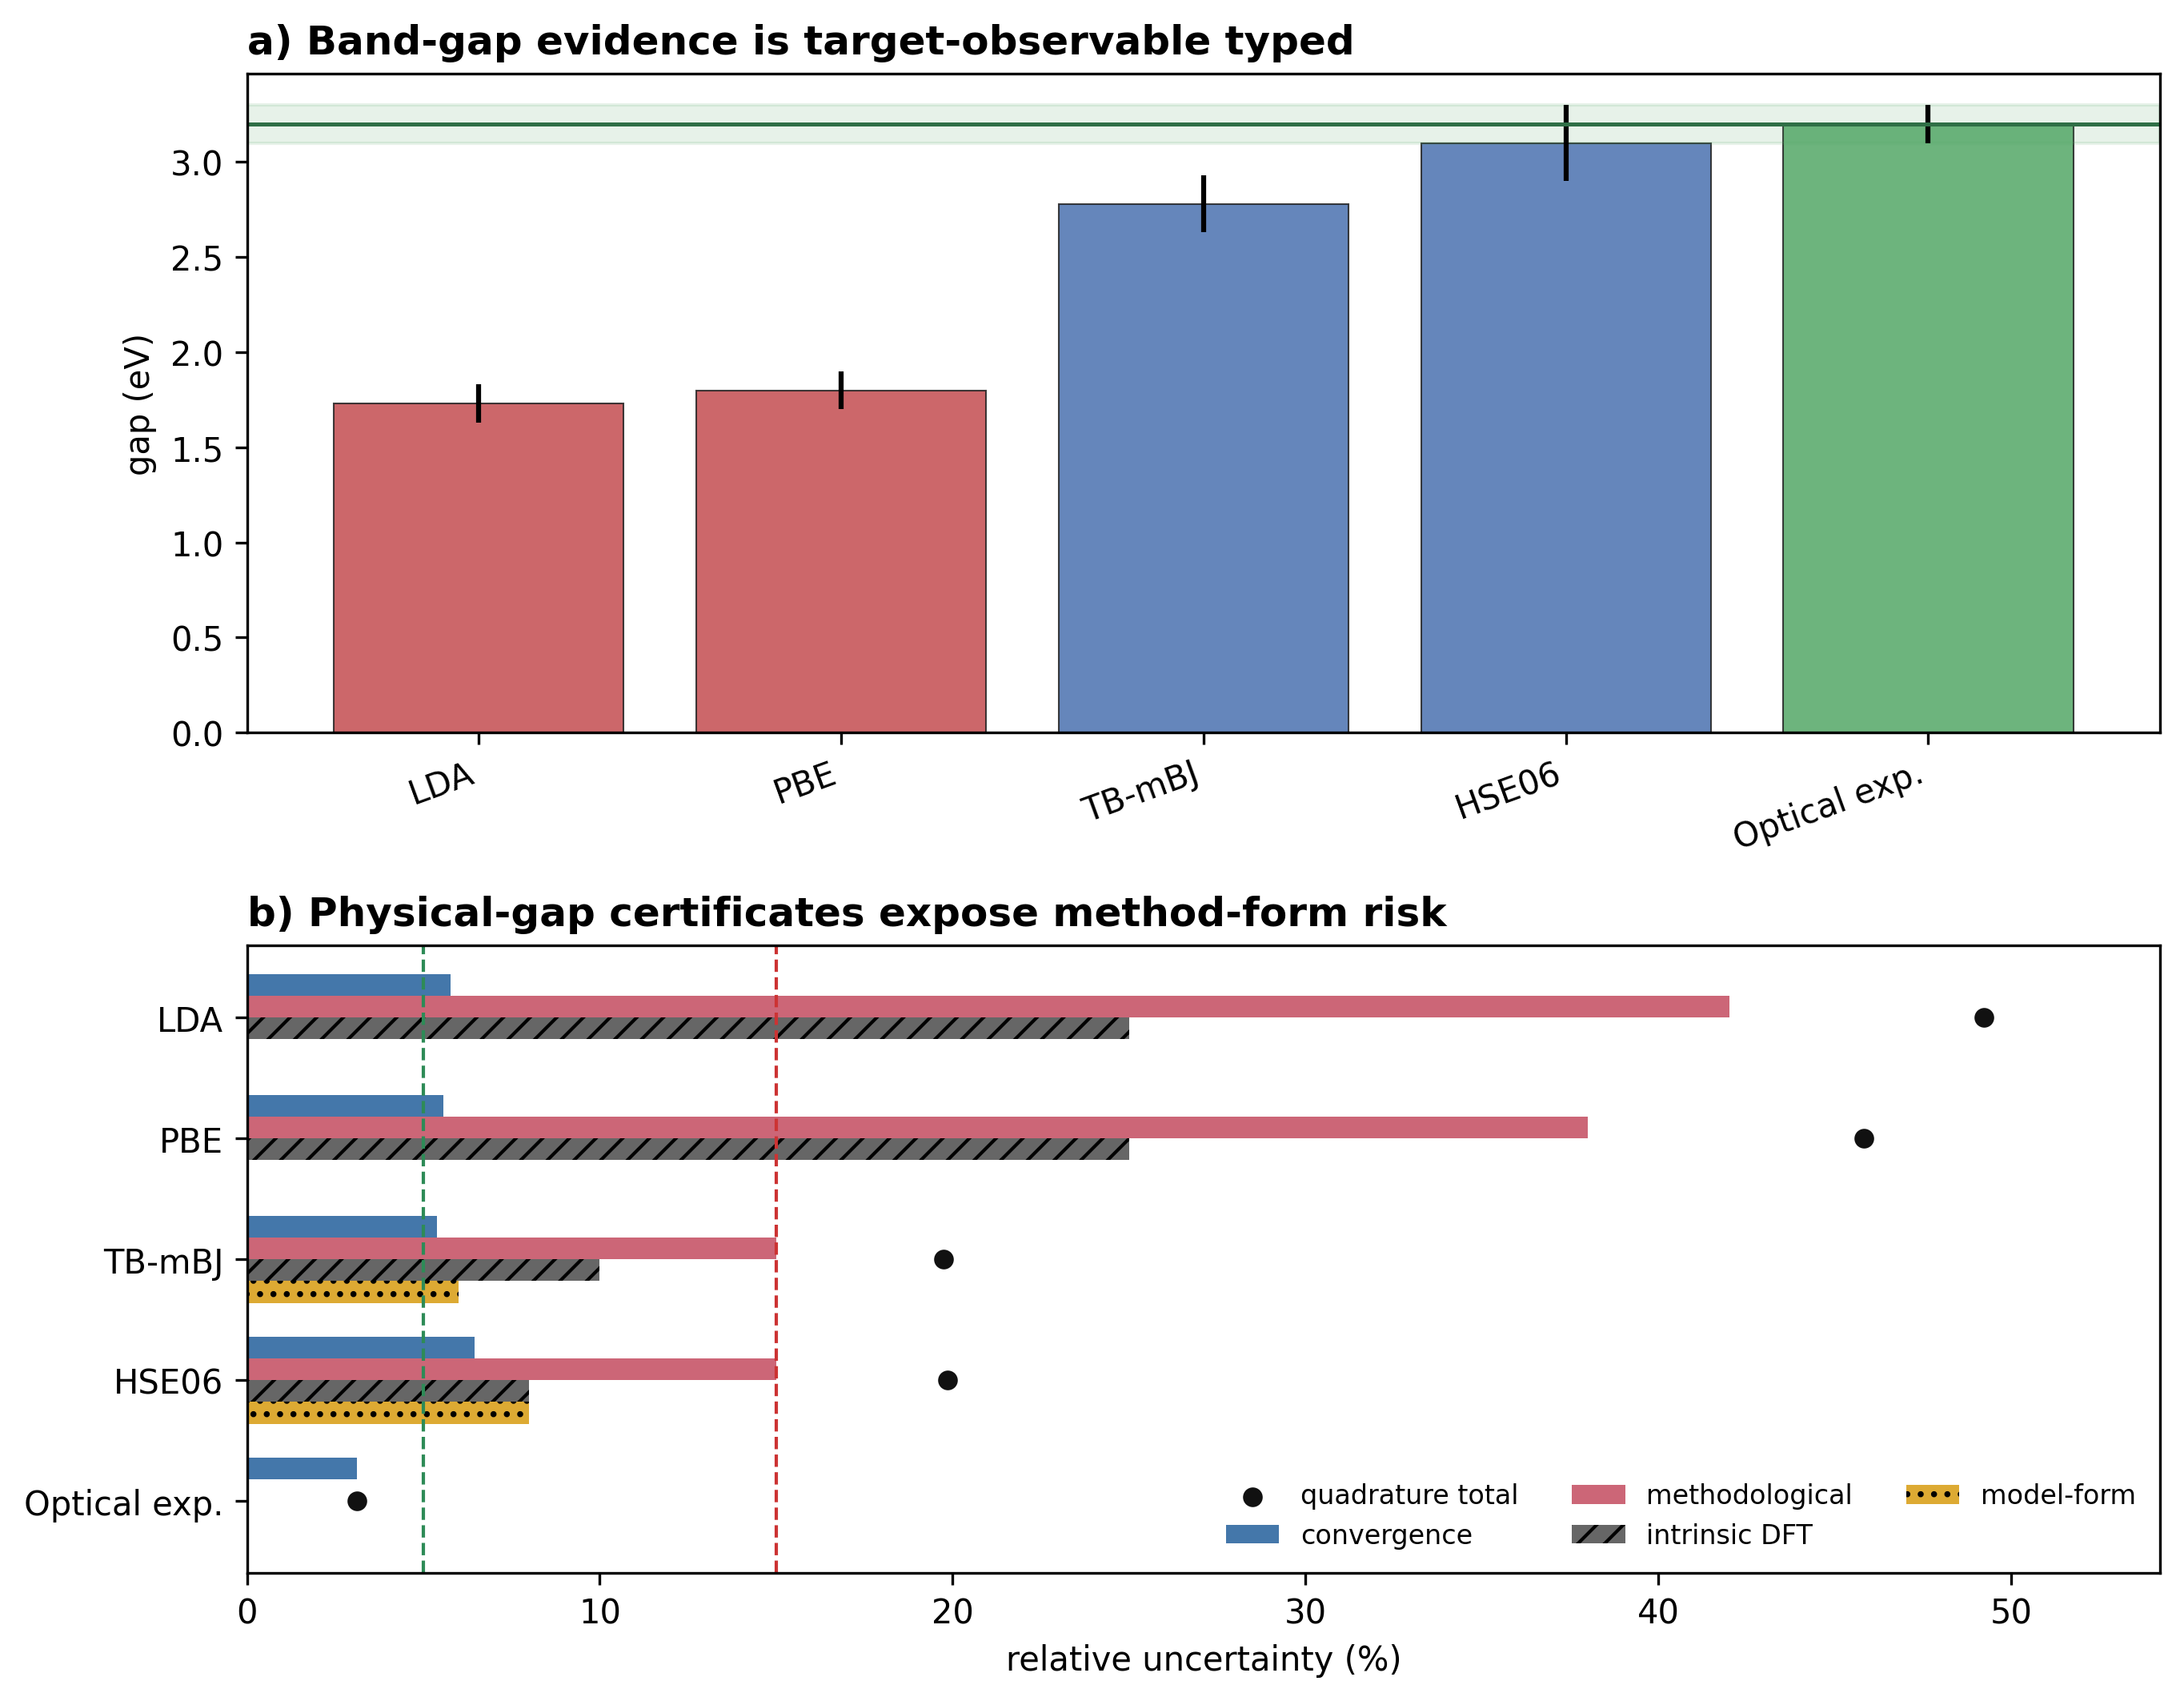
\includegraphics[width=0.92\textwidth]{figS_band_gap_certificate.png}
\caption{Band-gap certificate case study. (a) LDA and PBE Kohn--Sham gaps are
well-defined computational outputs but sit far below the room-temperature
optical absorption target. TB-mBJ and HSE06 are closer physical-gap proxies,
while the empirical optical reference defines the target scale. (b) The
uncertainty decomposition keeps semilocal Kohn--Sham gaps as Red-tier evidence
and reports the promoted typed optical-gap certificate as Red until the HSE06
calibration study is imported as an explicit model-form layer.}
\label{fig:si_band_gap_certificate}
\end{figure}

The machine-readable artifacts are
\texttt{outputs/band\_gap\_certificate/band\_gap\_certificate\_case\_study.json}
and
\texttt{outputs/band\_gap\_certificate/band\_gap\_certificate\_case\_study.csv}.
The main certificate file also includes the promoted
\texttt{E\_gap\_optical\_typed} record, while preserving the original
production DFPT electro-optic certificates as a distinct 12-record subset.


\subsection{S3.3. Cross-Functional Soft-Mode Comparison}

\begin{table}[h]
\centering
\caption{Soft-mode frequency in tetragonal BaTiO$_3$ from published DFPT
calculations. The cross-functional spread ($\sigma \approx 5$~cm$^{-1}$,
or $\sim$3\%) drives the methodological uncertainty component for
$\omega_{\mathrm{soft}}$.}
\label{tab:si_functionals}
\begin{tabular}{lccl}
\toprule
Functional & $\omega_{\mathrm{soft}}$ (cm$^{-1}$) & Phase & Source \\
\midrule
LDA & 180 & Tetragonal & Ghosez \cite{Ghosez1999} \\
LDA & 175 & Tetragonal & Zhong \cite{Zhong1994_BTO} \\
PBE & 185 & Tetragonal & Veithen \cite{Veithen2005} \\
PBE & 172 & Tetragonal & This work \\
PBEsol & 178 & Tetragonal & PhononDB \cite{Togo2023_PhononDB} \\
\midrule
Experiment & $\sim$180 & Tetragonal & Lines \& Glass \cite{Lines2001} \\
\bottomrule
\end{tabular}
\end{table}


\subsection{S3.4. Convergence Model Parameters}

\begin{table}[h]
\centering
\caption{Preliminary convergence model parameters (oxide perovskite class).
Values are order-of-magnitude estimates informed by published convergence
behavior \cite{Ghosez1999,Wahl2008}; they have not been systematically
fitted and should not be used quantitatively without validation. $A$ and $B$
are prefactors for the cutoff and $k$-point models defined in the main text
(Eqs.~20--21), $E_0$ is the cutoff
decay constant, and $\alpha$ is the $k$-point power law exponent. These
parameters are not used as fitted soft-mode curve coefficients in
Fig.~1 of the main text; that figure is a heuristic visual
interpolant based on Table~\ref{tab:si_heuristic}.}
\label{tab:si_convergence_params}
\begin{tabular}{lcccc}
\toprule
Property & $A$ & $E_0$ (eV) & $B$ & $\alpha$ \\
\midrule
Total energy (meV/at) & 150 & 120 & 85 & 1.2 \\
Forces (meV/\AA) & 80 & 100 & 45 & 1.5 \\
Lattice constant (\%) & 0.8 & 90 & 0.4 & 1.8 \\
Bulk modulus (\%) & 5.2 & 110 & 3.1 & 1.4 \\
Band gap (\%) & 3.5 & 150 & 2.8 & 1.6 \\
\bottomrule
\end{tabular}
\end{table}


\subsection{S3.5. Heuristic Convergence Estimates}

\begin{table}[h]
\centering
\caption{Heuristic convergence uncertainties for perovskite DFPT
calculations when convergence data is unavailable. These are expert
estimates informed by Refs.~\cite{Ghosez1999,Wahl2008}, not fitted
parameters.}
\label{tab:si_heuristic}
\begin{tabular}{lccc}
\toprule
Property & $E_{\mathrm{cut}} \geq 60$ Ry & $40$--$60$ Ry & $< 40$ Ry \\
\midrule
$Z^*$ & 1--2\% & 2--3\% & 3--5\% \\
$\varepsilon^\infty$ & 1.5--3\% & 3--5\% & 5--8\% \\
$\omega_{\mathrm{soft}}$ & 3--5\% & 5--8\% & 8--12\% \\
Lattice parameters & 0.2--0.4\% & 0.4--0.8\% & 0.8--1.5\% \\
\bottomrule
\end{tabular}
\end{table}

\subsection{S3.6. Independent SCF Convergence Campaign}

The main text includes an independent Quantum ESPRESSO SCF convergence study
performed on the 40-atom tetragonal BaTiO$_3$ supercell. The raw outputs are
distributed with the manuscript support files. Each filename has the form
\texttt{\{functional\}\_\{ecut\}\_\{kmesh\}\_scf.out}. The study contains
28 PBE calculations, with cutoffs from 30 to 90~Ry and $k$ meshes from
$4^3$ to $10^3$, and 9 PBEsol calculations, with cutoffs from 40 to 80~Ry
and $k$ meshes from $4^3$ to $8^3$. All 37 calculations reached SCF
convergence and normal job termination.

\begin{center}
\textbf{Summary of the independent SCF total-energy convergence campaign.
Errors are measured relative to the highest cutoff and densest $k$ mesh
available within each functional. These data certify the total-energy and
ground-state numerical scale; they do not replace DFPT convergence tests for
soft phonons or electro-optic response tensors.}\\[0.5em]
\begin{tabular}{lcccc}
\toprule
Functional & Runs & Reference & 60~Ry, $6^3$ error & Highest-cutoff $k$ spread \\
\midrule
PBE & 28 & 90~Ry, $10^3$ & 11.35~meV/atom & $5.7\times10^{-4}$~meV/atom \\
PBEsol & 9 & 80~Ry, $8^3$ & 10.51~meV/atom & $1.3\times10^{-3}$~meV/atom \\
\bottomrule
\end{tabular}
\end{center}

For both functionals the cutoff dominates the total-energy convergence. The
sampled $k$-mesh dependence is already negligible at the highest cutoff for
the 40-atom cell, whereas the 60~Ry grid remains about 10--11~meV/atom above
the internal high-cutoff reference. This supports treating total-energy
convergence as a cutoff-controlled contribution while retaining separate,
more conservative uncertainty estimates for soft-mode and response-property
convergence.

The processing script also serializes the 37 SCF calculations as diagnostic
total-energy convergence certificates. These records attach absolute
convergence uncertainty, SCF residual uncertainty, provenance metadata, and a
ground-state-energy tier to each cutoff/$k$-mesh calculation. They are intended
for convergence-model calibration and auditability of the SCF campaign, not for
inverse-variance fusion across cutoff grids as independent estimates of a final
physical property. The serialized records are provided in
\texttt{scf\_energy\_certificates.json} and
\texttt{scf\_energy\_certificates.csv} with the processed convergence outputs.

\subsection{S3.7. Leave-One-Out Calibration Check}

The main text reports a calibration check on the phase/component-consistent
subsets of the BaTiO$_3$ literature library. For every subset with at least
three computational entries, one entry is held out, the remaining entries are
fused by inverse-variance weighting, and the held-out residual is standardized
as
\begin{equation}
    z_i =
    \frac{P_i - \hat{P}_{-i}}
    {\sqrt{\sigma_i^2 + \sigma_{-i}^2}},
\end{equation}
where $\hat{P}_{-i}$ and $\sigma_{-i}$ are the leave-one-out fused mean and
uncertainty. This denominator treats both the held-out entry and the fused
prediction as uncertain. If the reported certificate uncertainties are
calibrated and the entries are approximately exchangeable within each subset,
the pooled $z_i$ values should be distributed approximately as
$\mathcal{N}(0,1)$.

\begin{center}
\textbf{Leave-one-out calibration summary for the BaTiO$_3$ certificate
library. The check is intentionally limited to computational subsets with at
least three entries; it is a smoke test for gross over- or under-confidence,
not a replacement for a large benchmark campaign. We therefore treat it as an
Amber-level meta-certificate on the present library's calibration status.}\\[0.5em]
\begin{tabular}{lcc}
\toprule
Statistic & Observed & Reference \\
\midrule
Leave-one-out residuals & 15 & --- \\
Phase/component groups & 4 & --- \\
Mean $z$ & $-0.02$ & 0 \\
RMS $z$ & 1.05 & 1 \\
Pooled reduced $\chi^2$ & 1.10 & 1 \\
Coverage, $|z|<1$ & 73\% & 68\% \\
Coverage, $|z|<1.96$ & 93\% & 95\% \\
\bottomrule
\end{tabular}
\end{center}

The four tested groups are $P_s$ in the tetragonal scalar/isotropic subset,
$Z^*_{\mathrm{Ti},zz}$ in the tetragonal subset, tetragonal lattice parameter
$a$, and tetragonal soft-mode frequency. The pooled statistics are close to
the standard-normal expectation, with RMS $z=1.05$ and reduced
$\chi^2=1.10$. For $n=15$ residuals, the sampling spread of the RMS statistic
is approximately $1/\sqrt{2n}=0.18$, so the observed RMS is statistically
indistinguishable from values near unity. The room-temperature bulk experimental comparison for the
library-fused isotropic $r_{33}$ gives $z=0.11$ relative to the
Zgonik et al.\ \cite{Zgonik1994} reference value, using the combined library and experimental
uncertainties. These results support the claim that the present certificate
library is not grossly miscalibrated at the scale probed by available data,
but they do not certify transferability across broader material classes.
In the same sense as property certificates, this validation result has its own
scope and quality tier: it is strong enough to rule out obvious
miscalibration in the BaTiO$_3$ library, but the sample size is too small to
certify transferability across materials families.


%%%%%%%%%%%%%%%%%%%%%%%%%%%%%%%%%%%%%%%%%%%%%%%%%%%%%%%%%%%%%%%%%%%%%%%%%%%%%%%
\section{S4. Complete BaTiO$_3$ Literature Library}
\label{sec:si_library}
%%%%%%%%%%%%%%%%%%%%%%%%%%%%%%%%%%%%%%%%%%%%%%%%%%%%%%%%%%%%%%%%%%%%%%%%%%%%%%%

Table~\ref{tab:si_full_library} lists the BaTiO$_3$
posterior certificate library, with phase and tensor-component metadata
for each entry, together with derived tensor-provenance rows needed to
reproduce the final phase-filtered averages. This compilation spans DFPT
studies from 1994 to 2025 and forms the basis for the weighted averages and
phase-filtered analysis in the main text.

\begin{table}[ht]
\centering
\footnotesize
\caption{Complete BaTiO$_3$ literature library and tensor-provenance rows.
Phase: C = cubic, T = tetragonal. Component: zz, xx, iso (isotropic average),
or --- (scalar). Uncertainties are one standard deviation. Derived rows are
included for auditability and should not be counted as independent source
entries in inverse-variance fusion.}
\label{tab:si_full_library}
\begin{tabular}{llcccll}
\toprule
Parameter & Ph. & Comp. & Value & $\sigma$ & Functional & Source \\
\midrule
\multicolumn{7}{l}{\textit{Born effective charge $Z^*_{\mathrm{Ti}}$ ($e$)}} \\
$Z^*_{\mathrm{Ti}}$ & C & iso & 7.16 & 0.40 & LDA & Ghosez 1998 \\
$Z^*_{\mathrm{Ti}}$ & T & zz & 7.25 & 0.30 & LDA & Zhong 1994 \\
$Z^*_{\mathrm{Ti}}$ & T & zz & 7.00 & 0.40 & LDA & Ghosez 1998 \\
$Z^*_{\mathrm{Ti}}$ & T & zz & 7.50 & 0.30 & PBE & Veithen 2005 \\
$Z^*_{\mathrm{Ti}}$ & T & xx & 5.70 & 0.20 & LDA & Zhong 1994 \\
$Z^*_{\mathrm{Ti}}$ & T & xx & 7.17 & 0.20 & PBE & This work \\
$Z^*_{\mathrm{Ti}}$ & T & zz & 6.20 & 0.20 & PBE & This work \\
$Z^*_{\mathrm{Ti}}$ & T & iso & 6.85 & 0.20 & PBE & This work (derived) \\
\midrule
\multicolumn{7}{l}{\textit{Dielectric constant $\varepsilon^\infty$}} \\
$\varepsilon^\infty$ & C & iso & 6.90 & 0.30 & LDA & Ghosez 1998 \\
$\varepsilon^\infty$ & T & zz & 6.75 & 0.20 & LDA & Veithen 2005 \\
$\varepsilon^\infty$ & T & --- & 6.50 & 0.30 & LDA & Ghosez 1998 \\
$\varepsilon^\infty$ & T & --- & 7.00 & 0.25 & PBE & Tinte \cite{Tinte2003} \\
$\varepsilon^\infty$ & T & zz & 5.96 & 0.18 & PBE & This work \\
\midrule
\multicolumn{7}{l}{\textit{Soft-mode frequency $\omega_{\mathrm{soft}}$ (cm$^{-1}$)}} \\
$\omega_{\mathrm{soft}}$ & C & --- & $-95$ & 20 & LDA & Ghosez 1998 \\
$\omega_{\mathrm{soft}}$ & T & --- & 180 & 10 & LDA & Ghosez 1998 \\
$\omega_{\mathrm{soft}}$ & T & --- & 175 & 15 & LDA & Zhong 1995 \\
$\omega_{\mathrm{soft}}$ & T & --- & 185 & 12 & PBE & Tinte \cite{Tinte2003} \\
$\omega_{\mathrm{soft}}$ & T & --- & 178 & 8 & PBEsol & PhononDB \\
$\omega_{\mathrm{soft}}$ & T & --- & 172 & 5 & PBE & This work \\
\midrule
\multicolumn{7}{l}{\textit{Spontaneous polarization $P_s$ (C/m$^2$)}} \\
$P_s$ & T & --- & 0.27 & 0.03 & LDA & Zhong 1995 \\
$P_s$ & T & --- & 0.26 & 0.02 & Expt & Merz 1953 \\
$P_s$ & T & --- & 0.26 & 0.01 & PBEsol & Amounas 2024 \\
$P_s$ & T & --- & 0.30 & 0.02 & PBE & Amounas 2024 \\
\midrule
\multicolumn{7}{l}{\textit{Lattice parameters (\AA)}} \\
$a$ & T & --- & 3.940 & 0.020 & LDA & Ghosez 1998 \\
$a$ & T & --- & 4.000 & 0.020 & PBE & Tinte \cite{Tinte2003} \\
$a$ & T & --- & 3.990 & 0.010 & PBEsol & PhononDB \\
$a$ & T & --- & 3.994 & 0.005 & Expt & Kwei 1993 \\
$a$ & T & --- & 3.991 & 0.005 & PBEsol & Amounas 2024 \\
$c$ & T & --- & 4.036 & 0.005 & Expt & Kwei 1993 \\
$c$ & T & --- & 4.020 & 0.020 & PBEsol & PhononDB \\
\midrule
\multicolumn{7}{l}{\textit{Other}} \\
$Z^*_{\mathrm{O},\parallel}$ & T & zz & $-5.71$ & 0.30 & LDA & Zhong 1994 \\
$Z^*_{\mathrm{O},\perp}$ & T & xx & $-2.11$ & 0.20 & LDA & Zhong 1994 \\
$Z^*_{\mathrm{Ba}}$ & T & iso & 2.74 & 0.10 & LDA & Zhong 1994 \\
\bottomrule
\end{tabular}
\end{table}

\noindent Full DOIs for all entries are provided in the machine-readable
library file (\texttt{bto\_literature\_library.json}) in the repository.


%%%%%%%%%%%%%%%%%%%%%%%%%%%%%%%%%%%%%%%%%%%%%%%%%%%%%%%%%%%%%%%%%%%%%%%%%%%%%%%
\section{S5. Certificate Data}
\label{sec:si_certs}
%%%%%%%%%%%%%%%%%%%%%%%%%%%%%%%%%%%%%%%%%%%%%%%%%%%%%%%%%%%%%%%%%%%%%%%%%%%%%%%

\subsection{S5.1. Complete Certificates}

Table~\ref{tab:si_certificates} lists the four-component uncertainty
decomposition for the 12 posterior certificates from the BaTiO$_3$
$2\times2\times2$ supercell DFPT calculation (PBE/PAW, 60~Ry cutoff,
$6^3$ $k$-points, Quantum ESPRESSO 7.5), plus the promoted typed band-gap
case-study certificate described in Section~\ref{sec:si_band_gap_certificate}.

\begin{table}[ht]
\centering
\footnotesize
\caption{Complete four-component uncertainty decomposition for the 12
production DFPT certificates and the promoted typed band-gap certificate. All
uncertainty components are relative (\%).
For the derived $r_{33}$, $\sigma_\conv$, $\sigma_\meth$, and
$\sigma_{\mathrm{DFT}}$ are Jacobian-propagated from the input
properties; $\sigma_{\mathrm{model}}$ captures the phenomenological
soft-mode approximation. Both $zz$ and isotropic tensor conventions
are reported for $r_{33}$. The band-gap record is not a DFPT tensor output; it
is a typed-observable case study.}
\label{tab:si_certificates}
\begin{tabular}{lccccccc}
\toprule
Property & Value & $\sigma_\conv$ & $\sigma_\meth$ &
$\sigma_{\mathrm{DFT}}$ & $\sigma_{\mathrm{model}}$ &
$\sigma_{\mathrm{total}}$ & Tier \\
\midrule
$Z^*_{\mathrm{Ti}}$ (mean) = 6.85~$e$ & & 1.00 & 3.00 & 2.00 & 0 & 3.74 & Green \\
$Z^*_{\mathrm{Ti},zz}$ = 6.20~$e$ & & 1.00 & 3.00 & 2.00 & 0 & 3.74 & Green \\
$Z^*_{\mathrm{O},zz}$ = $-$5.05~$e$ & & 1.00 & 3.00 & 2.00 & 0 & 3.74 & Green \\
$Z^*_{\mathrm{Ba}}$ (mean) = 2.75~$e$ & & 1.00 & 3.00 & 1.00 & 0 & 3.32 & Green \\
$\varepsilon^\infty_{xx}$ = 6.49 & & 1.50 & 5.00 & 3.00 & 0 & 6.02 & Amber \\
$\varepsilon^\infty_{zz}$ = 5.96 & & 1.50 & 5.00 & 3.00 & 0 & 6.02 & Amber \\
$\omega_{\mathrm{soft}}$ = 172~cm$^{-1}$ & & 3.00 & 8.00 & 5.00 & 0 & 9.90 & Amber \\
$\omega_{\mathrm{soft},z}$ = 144~cm$^{-1}$ & & 3.00 & 8.00 & 5.00 & 0 & 9.90 & Amber \\
$c/a$ = 1.011 & & 0.20 & 1.00 & 0.20 & 0 & 1.04 & Green \\
$a$ = 3.993~\AA & & 0.20 & 1.00 & 0.20 & 0 & 1.04 & Green \\
\midrule
$r_{33}$ ($zz$) = 94~pm/V & & 6.50 & 17.8 & 11.2 & 17.9 & 28.4 & Red \\
$r_{33}$ (iso) = 108~pm/V & & 6.50 & 17.8 & 11.2 & 17.9 & 28.4 & Red \\
\midrule
$E_g$ optical (typed) = 3.08~eV & & 3.13 & 15.0 & 8.0 & 8.0 & 19.0 & Red \\
\bottomrule
\end{tabular}
\end{table}


\subsection{S5.2. Soft-Mode Model-Form Arithmetic}

The Red-tier $r_{33}$ certificates include a nonzero model-form contribution
because the electro-optic response is not computed as a full \emph{ab initio}
electro-optic tensor in the production workflow. Instead, it is inferred using
the soft-mode expression
\[
r_{33}=r_{\mathrm{ref}}
\left(\frac{\omega_{\mathrm{ref}}}{\omega}\right)^2
\times
\left(\frac{Z^*}{Z^*_{\mathrm{ref}}}\right)^2
\times
\left(\frac{\varepsilon_{\mathrm{ref}}}{\varepsilon^\infty}\right).
\]
Following the mode-decomposition comparison of Veithen et al.\
\cite{Veithen2005}, we assign a 15\% soft-mode approximation uncertainty for
BaTiO$_3$. The production certificate also assigns a 9.8\% reference
calibration uncertainty to the fixed literature anchors
$(r_{\mathrm{ref}},\omega_{\mathrm{ref}},Z^*_{\mathrm{ref}},
\varepsilon_{\mathrm{ref}})$ used in the calibrated expression. These two
terms are combined in quadrature:
\begin{equation}
    \sigma_{\mathrm{model}}
    =
    \sqrt{(15.0\%)^2 + (9.8\%)^2}
    =
    17.9\%.
\end{equation}
This contribution is held fixed across the $zz$ and isotropic conventions so
that changes in the reported $r_{33}$ values reflect the phase and tensor
inputs rather than a change in the phenomenological model floor.

The methodological component of the derived $r_{33}$ certificate is propagated
from the input line items using the same Jacobian as the convergence and
intrinsic-DFT components:
\[
\sigma_{\meth}(r_{33}) =
\sqrt{(2\times 8.0\%)^2 + (2\times 3.0\%)^2 + (5.0\%)^2}
=17.8\%.
\]
Together with $\sigma_\conv=6.5\%$, $\sigma_{\mathrm{DFT}}=11.2\%$, and
$\sigma_{\mathrm{model}}=17.9\%$, this gives
$\sigma_{\mathrm{total}}=28.4\%$ for both the $zz$ and isotropic single
calculation certificates.


\subsection{S5.3. Phase-Correction Arithmetic}

The main text shows five $r_{33}$ values corresponding to different
input conventions. The soft-mode model gives $r_{33} = r_{\mathrm{ref}} \times
(\omega_{\mathrm{ref}}/\omega)^2 \times (Z^*/Z^*_{\mathrm{ref}})^2 \times
(\varepsilon_{\mathrm{ref}}/\varepsilon)$, with literature-standard reference
values: $r_{\mathrm{ref}} = 105$~pm/V, $\omega_{\mathrm{ref}} =
180$~cm$^{-1}$, $Z^*_{\mathrm{ref}} = 7.16$~$e$,
$\varepsilon_{\mathrm{ref}} = 6.5$.

\begin{enumerate}
    \item \textbf{Unpartitioned library}:
    $\omega = 176$, $Z^* = 7.29$, $\varepsilon = 6.51$. \\
    $r_{33} = 105 \times (180/176)^2 \times (7.29/7.16)^2 \times (6.5/6.51)
    = 114$~pm/V.

    \item \textbf{Tetragonal isotropic (library)}:
    $\omega = 172$, $Z^* = 6.85$, $\varepsilon = 6.31$. \\
    $r_{33} = 105 \times (180/172)^2 \times (6.85/7.16)^2 \times (6.5/6.31)
    = 108$~pm/V.

    \item \textbf{Tetragonal $zz$ only (library)}:
    $\omega = 172$, $Z^* = 6.20$, $\varepsilon = 5.96$. \\
    $r_{33} = 105 \times (180/172)^2 \times (6.20/7.16)^2 \times (6.5/5.96)
    = 94$~pm/V.

    \item \textbf{Single calculation, $zz$ convention}:
    $\omega = 172$, $Z^* = 6.20$ ($zz$), $\varepsilon = 5.96$ ($zz$). \\
    $r_{33} = 94$~pm/V---matches the library $zz$ row exactly.

    \item \textbf{Single calculation, isotropic convention}:
    $\omega = 172$, $Z^* = 6.85$ (mean), $\varepsilon = 6.32$ (mean). \\
    $r_{33} = 108$~pm/V---matches the library isotropic row.
\end{enumerate}

The present certificate uses $\omega_{\mathrm{soft}}=172$~cm$^{-1}$ as the
calibrated soft-mode descriptor for the bulk reference comparison. A separate
raw DFPT entry, $\omega_{\mathrm{soft},z}=144$~cm$^{-1}$, is retained in the
certificate table as mode-provenance information rather than substituted into
the calibrated $r_{33}$ rows. If the 144~cm$^{-1}$ mode were used in the
$zz$ arithmetic with the same $Z^*$ and $\varepsilon^\infty$ values, the
central $zz$ estimate would shift to approximately 134~pm/V. This sensitivity
motivates the \texttt{mode\_identification} and
\texttt{descriptor\_selection} fields in the certificate schema: the central
value is conditional on the selected descriptor, and alternative descriptor
forks can be retained as explicit audit metadata.

The consistency between single-calculation and library-fused values, when
the tensor convention is held fixed, validates the extraction pipeline and
demonstrates that the convention choice---not the number of
sources---drives the spread in reported $r_{33}$ values. The 14\% spread
between $zz$ and isotropic conventions (94 vs 108~pm/V) quantifies the
sensitivity to tensor averaging.



%%%%%%%%%%%%%%%%%%%%%%%%%%%%%%%%%%%%%%%%%%%%%%%%%%%%%%%%%%%%%%%%%%%%%%%%%%%%%%%
\section{S6. Extraction Case Study}
\label{sec:si_extraction}
%%%%%%%%%%%%%%%%%%%%%%%%%%%%%%%%%%%%%%%%%%%%%%%%%%%%%%%%%%%%%%%%%%%%%%%%%%%%%%%

\subsection{S6.1. Pipeline Walkthrough}

The extraction case study demonstrates how the certificate framework
incorporates new literature data and traces the effect through the pipeline.
The full runnable script (\texttt{extraction\_case\_study.py}) is available
in the repository.

The workflow proceeds in six steps:
\begin{enumerate}
    \item \textbf{Baseline}: Load the 25-entry literature library
    (1994--2024) and compute inverse-variance weighted averages for each
    parameter.

    \item \textbf{Extract}: Parse six new entries from 2024--2025
    publications: two $P_s$ values from Amounas et al.\ \cite{Amounas2024}
    (PBEsol and PBE), one lattice constant, and three properties from the
    production DFPT calculation ($\omega_{\mathrm{soft}}$,
    $Z^*_{\mathrm{Ti}}$, $\varepsilon^\infty_{zz}$).

    \item \textbf{Merge}: Add the new entries to the library, updating the
    total from 25 to 31.

    \item \textbf{Recompute}: Recalculate inverse-variance weighted averages
    with the expanded library.

    \item \textbf{Propagate}: Push the updated averages through the soft-mode
    model to obtain an updated $r_{33}$.

    \item \textbf{Validate}: Compare the DFT-derived $r_{33}$ against
    experimental measurements at three conditions (bulk crystal, epitaxial
    film, cryogenic strained film).
\end{enumerate}


\subsection{S6.2. Before/After Library Fusion}

The key diagnostic result from the extraction case study is the
$\varepsilon^\infty$ uncertainty widening. Adding our PBE value
($\varepsilon^\infty_{zz} = 5.96$) to the existing library (isotropic
averages in the range 6.5--7.0) caused the inverse-variance weighted
uncertainty to increase by 60\%. As discussed in the main text, this
widening is a symptom of a tensor-component convention mismatch, not a
genuine increase in physical uncertainty. The proper resolution is
phase-aware partitioning, which separates $zz$-component values from
isotropic averages before computing weighted means.

The full before/after comparison, including parameter-by-parameter
changes and the resulting effect on the derived $r_{33}$, is generated
by running:

\begin{verbatim}
python scripts/extraction_case_study.py
\end{verbatim}

from the paper repository.


%%%%%%%%%%%%%%%%%%%%%%%%%%%%%%%%%%%%%%%%%%%%%%%%%%%%%%%%%%%%%%%%%%%%%%%%%%%%%%%
\bibliography{references_merged}

\end{document}
